\chapter{Stochastic Models and Martingale Duality}\label{chap:stochastic}

The previous chapter proved that a uniformly random residue modulo $2^k$
produces a parity vector\index{parity vector} of $k$ independent fair coin flips. It is a short
step from this theorem to a model: pretend that the parities along an orbit
are fair coin flips forever, and study the resulting random walk for $\log x$.
The model rests on this theorem of Terras\index{Terras, R.}~\cite{terras1976} and Everett\index{Everett, C. J.}~\cite{everett1977} and was stated as a heuristic by Crandall\index{Crandall, R. E.}~\cite{crandall1978} (\cref{sec:ch3:heuristic} tells its history).
Its predictions agree closely with computation (the fitted slope of the total stopping times to within about two percent over the ranges tested, and to within half a percent for the accelerated map below $10^4$; their variance to about ten percent), and it is the reason almost everyone who has thought about the problem believes the conjecture.

This chapter develops the model with the tools of martingale\index{martingale} theory. The
organizing fact is a duality. Under the fair coin model for the accelerated
map, the iterates $x_n$ themselves form a martingale, because
$\tfrac12\cdot\tfrac12+\tfrac12\cdot\tfrac32=1$ exactly, while their
logarithms form a supermartingale\index{supermartingale} with strictly negative drift\index{drift}
$\ds=\log(\sqrt3/2)\approx-0.1438$. The two statements are reconciled by
Jensen's inequality\index{Jensen inequality}, and the drift is exactly the Jensen gap.
The heuristic is therefore not a statement about the size of the iterates on average, which in the model does not decrease at all, but about the size of their logarithms.
Almost everything else in the chapter follows from this observation: the total stopping
time slope $1/|\ds|\approx6.952$ through Wald's identity\index{Wald identity}, the dispersion of
total stopping times\index{stopping time} through the central limit theorem\index{central limit theorem} and the moment asymptotics for first passage times, a
bound of exactly $1/K$ on the probability of an excursion by a factor $K$
through Ville\index{Ville inequality}'s maximal inequality, absorption with probability one, and the
failure of uniform integrability\index{uniform integrability} that prevents the martingale from saying
anything about where the orbit ends. We also treat the standard map\index{standard map} $T_0$,
whose model parity sequence is not independent but a renewal\index{renewal theory} sequence, and we
compute its autocorrelation\index{autocorrelation} function exactly: $\rho(h)=(-\tfrac12)^h$.

Apart from \cref{prop:ch3:exact,prop:ch3:pathwise}, which are statements about the map, every result in this chapter is a theorem about a probabilistic model, and the
model is not the Collatz map. We say so at the start because the point is easy
to lose in the middle of a computation. The final section asks what a proof of
the conjecture along these lines would have to supply, and the answer, a
certificate\index{certificate} that transfers the model's conclusions to individual orbits, is
the subject of much of the rest of the book.

\section{The parity heuristic}\label{sec:ch3:heuristic}

\subsection{From Terras to Lagarias and Weiss}

Terras\index{Terras, R.}~\cite{terras1976} and, independently, Everett\index{Everett, C. J.}~\cite{everett1977}
introduced the parity vector\index{parity vector} and proved that its first
$k$ entries are uniformly distributed when the starting value is uniformly
distributed modulo $2^k$ (\cref{thm:terras}; see \cite[Theorem~B]{lagarias1985}),
and both proved that almost all integers have a finite stopping time
(the density statement of \cref{thm:density}, whose exponential rate is due to Lagarias\index{Lagarias, J. C.}~\cite[Theorem~D]{lagarias1985}; see also~\cite{terras1979}). Both papers use the coin flip
picture to prove theorems about densities of starting values, and both are
careful to stay within the range of steps that the residue class actually
controls. The heuristic consists in ignoring that limitation.

The heuristic was stated explicitly by Crandall\index{Crandall, R. E.}~\cite{crandall1978}.
Lagarias\index{Lagarias, J. C.}, in his 1985 survey~\cite[\S2.1]{lagarias1985}, recorded it
and pointed out that it predicts the growth rate of total stopping times\index{stopping time}.
Lagarias and Weiss\index{Weiss, A.}~\cite{lagarias1992} then studied two stochastic models in
detail, a random walk model for the trajectory of a single integer and a
branching random walk model for the tree of preimages, and compared their
predictions for total stopping times and maximal excursions with extensive
computation. Kontorovich\index{Kontorovich, A. V.} and Sinai\index{Sinai, Ya. G.}~\cite{kontorovich2002} proved a structure
theorem for a broad family of maps of Collatz type, showing that the
logarithm of a trajectory from a random starting value behaves like a random
walk with drift\index{drift}; and the survey of Kontorovich and
Lagarias~\cite{kontorovich2009} places all of this, together with the $5x+1$
problem, where the drift is positive and orbits are expected to diverge, in a
common framework.

We shall use three versions of the model, one for each of the maps of
\cref{def:maps}. Throughout the chapter the multiplicative factor $3+1/x$ is
replaced by $3$; we comment on this replacement in
\cref{rem:ch3:plusone}.

\begin{definition}[Three stochastic models]\label{def:ch3:models}
\leavevmode
\begin{enumerate}[label=(\alph*),leftmargin=2em]
\item \emph{Bernoulli model for $T$.} Let $\xi_1,\xi_2,\ldots$ be independent
  with $\Prob(\xi_i=\tfrac12)=\Prob(\xi_i=\tfrac32)=\tfrac12$, and put
  $x_n=x_0\xi_1\cdots\xi_n$. The log increments are $\Delta_i=\log\xi_i$, and
  $\Filt_n=\sigma(\xi_1,\ldots,\xi_n)$.
\item \emph{Stride model for $S$.} Let $K_1,K_2,\ldots$ be independent,
  each with the Geometric$(\tfrac12)$ law, so that $\Prob(K_j=k)=2^{-k}$ for
  $k\geq1$, and put $X_j=X_{j-1}\cdot3\cdot2^{-K_j}$.
\item \emph{Renewal model for $T_0$.} Let $(B_n)_{n\geq0}$ be the Markov chain
  on $\{0,1\}$ with transition probabilities
  \begin{gather*}
    \Prob(B_{n+1}=0\mid B_n=1)=1,\\
    \Prob(B_{n+1}=0\mid B_n=0)=\Prob(B_{n+1}=1\mid B_n=0)=\tfrac12,
  \end{gather*}
  and put $x_{n+1}=3x_n$ if $B_n=1$ and $x_{n+1}=x_n/2$ if $B_n=0$. Here
  $B_n$ is the model counterpart of the parity $b_n=T_0^{(n)}(x_0)\bmod2$ of an
  orbit (\cref{prop:nocons}), and $\Filt_n=\sigma(B_0,\ldots,B_n)$.
\end{enumerate}
\end{definition}

The three models are consistent with one another in the same way the three maps
are. In model (c) an odd step is always followed by a halving, by
\cref{prop:nocons}; merging each odd step with the halving that follows it
produces a step with factor $3/2$, and the parity after that is again a fair
coin, so model (c) with the forced steps deleted is model (a). Grouping the
steps of model (a) into runs that begin with a factor $\tfrac32$ and continue
with factors $\tfrac12$ until the next $\tfrac32$ produces the factor
$3\cdot2^{-K}$ with $K$ Geometric$(\tfrac12)$, which is model (b). The three
models therefore describe one random path measured against three clocks, which
tick on average three times, twice and once per stride.

\subsection{In what sense the model is exact}

The model is not an analogy chosen for convenience. Over an initial segment of
the orbit whose length is controlled by the size of the starting residue class
it is exact, up to the replacement of $3+1/x$ by $3$.

\begin{proposition}[Ensemble exactness]\label{prop:ch3:exact}
Let $k\geq1$ and let $n$ be uniformly distributed on a complete set of residues
modulo $2^k$ consisting of positive integers. Then the parities of $T^{(j)}(n)$
for $0\leq j<k$ are independent and fair, and for $j\leq k$
\[
  \log T^{(j)}(n)-\log n=\sum_{i=1}^{j}\Delta_i+\sum_{\substack{0\le i<j\\
  T^{(i)}(n)\ \mathrm{odd}}}\log\Bigl(1+\frac{1}{3T^{(i)}(n)}\Bigr),
\]
where $\Delta_{i+1}=\log\frac32$ if $T^{(i)}(n)$ is odd and $\Delta_{i+1}=-\log2$
otherwise. Thus the first $k$ log increments of $T$ have exactly the joint law
of the increments of the Bernoulli model\index{Bernoulli model}, apart from correction terms that are
positive and at most $1/(3T^{(i)}(n))$ each.
\end{proposition}

\begin{proof}
The first statement is \cref{cor:ch2:iid}. The second is the identity
$T(x)/x=\tfrac32(1+\tfrac1{3x})$ for odd $x$ and $T(x)/x=\tfrac12$ for even
$x$, summed along the orbit.
\end{proof}

\Cref{prop:ch3:exact} is the source of the model's authority and also of its
limitation. A starting value $n$ of size about $2^k$ carries $k$ bits, and the
first $k$ steps of its orbit consume them, one bit per step. After that the
parities are a deterministic function of information that the orbit itself
has generated, and no theorem says that they continue to look like coin flips.
Since an orbit from $n$ needs about $\log n/|\ds|\approx4.8\log_2n$ steps of
$T$ to reach $1$ (\cref{prop:lyapunov}), roughly four fifths of a typical orbit lies beyond the range
where the model is a theorem.

\begin{remark}[The plus one]\label{rem:ch3:plusone}
Replacing $3+1/x$ by $3$ changes each odd step by a factor
$1+1/(3x)$, so the cumulative effect on $\log x$ along an orbit is
at most $\sum1/(3x_i)$ over its odd steps, which is negligible unless the orbit lingers at small
values. The replacement matters in two places only. Near the end of an orbit
it decides whether the path lands on the cycle $1\to2\to1$ under $T$, which the
multiplicative model cannot see. And it is the whole difference between the
$3x+1$ map and its multiplicative caricature, in which an exact return to a
previous value would require $3^m=2^k$; the cycle analysis of
\cref{chap:cycles} lives entirely in the $+1$. For questions of drift\index{drift}, dispersion and excursion, which are the
subject of this chapter, it is harmless.
\end{remark}

\section{Martingale duality}\label{sec:ch3:duality}

We begin with the accelerated map\index{accelerated map}, where the model is simplest.

\begin{proposition}[Martingale duality]\label{thm:martingale}
In the Bernoulli model\index{Bernoulli model} for the accelerated map $T$:
\begin{enumerate}[label=(\roman*),leftmargin=2em]
\item \emph{Multiplicative martingale.} $\E[\xi_i]=\tfrac12\cdot\tfrac12+
  \tfrac12\cdot\tfrac32=1$, so $(x_n)$ is a nonnegative martingale with
  $\E[x_n]=x_0$ for every $n$.
\item \emph{Log supermartingale.} $\E[\Delta_i]=\tfrac12\log\tfrac32-\tfrac12\log2
  =\log\frac{\sqrt3}{2}=\ds\approx-0.1438$, so $(\log x_n)$ is a strict
  supermartingale\index{martingale}\index{supermartingale}, and $\log x_n-n\ds$ is a martingale.
\item \emph{Wald root.} The moment generating function of the increment,
  \[
    M(\theta)=\E\bigl[e^{\theta\Delta_i}\bigr]=\tfrac12\,2^{-\theta}+
    \tfrac12\bigl(\tfrac32\bigr)^{\theta},
  \]
  is strictly convex with $M(0)=M(1)=1$. Its nonzero root
  $\theta^*$ of $M(\theta)=1$ is $\theta^*=1$, and $x_n^{\theta}$ is a
  supermartingale for $0\le\theta\le1$ and a submartingale for $\theta\geq1$
  or $\theta\le0$.
\item \emph{Jensen gap.} $\ds=\E[\log\xi_i]-\log\E[\xi_i]$, so the drift of
  $\log x_n$ is exactly the Jensen defect of the logarithm at the law of
  $\xi_i$.
\end{enumerate}
\end{proposition}

\begin{proof}
Parts (i) and (ii) are the two displayed computations together with the
independence of $\xi_{n+1}$ from $\Filt_n$: $\E[x_{n+1}\mid\Filt_n]=x_n\E[\xi_{n+1}]
=x_n$ and $\E[\log x_{n+1}\mid\Filt_n]=\log x_n+\ds$. For (iii),
$M(0)=1$ and $M(1)=\tfrac14+\tfrac34=1$. Since $M''(\theta)=\E[\Delta^2e^{\theta
\Delta}]>0$, $M$ is strictly convex, so it equals $1$ at exactly two points and
is below $1$ strictly between them and above $1$ outside. Finally
$\E[x_{n+1}^\theta\mid\Filt_n]=x_n^\theta M(\theta)$. Part (iv) restates (ii)
using $\log\E[\xi_i]=0$ from (i).
\end{proof}

Parts (i) and (ii) of \cref{thm:martingale} appear to contradict each other. By (i) the expected size of $x_n$ never
changes. By (ii) and the strong law of large numbers, $\log x_n/n\to\ds<0$
almost surely, so almost every path tends to zero exponentially fast, at the
rate $e^{n\ds}=(\sqrt3/2)^n$. Both are true. The mean is held up by rare paths
that grow enormously, and the typical path has nothing to do with the mean.
This is the familiar behaviour of a product of independent positive factors
with mean one, the same mechanism by which a fair multiplicative bet ruins
almost every gambler while preserving the expected wealth of the population.

\begin{remark}[Size of the Jensen gap]\label{rem:ch3:jensen}
The factor $\xi$ has mean $1$ and variance $\E\xi^2-1=\tfrac12(\tfrac14+\tfrac94)
-1=\tfrac14$. The second order expansion $\E\log\xi\approx\log\E\xi-
\Var(\xi)/(2(\E\xi)^2)$ gives $-\tfrac18=-0.125$, against the exact value
$\ds=-0.1438$.
The two values are symmetric about $1$, so the odd moments of $\xi-1=\pm\tfrac12$ vanish and $\E\log\xi=-\sum_{j\geq1}4^{-j}/(2j)=\tfrac12\log\tfrac34$; the second order value $-\tfrac18$ is the first term of this series, and the difference comes from the higher even moments.
Thus the descent of a Collatz orbit, in the model, is a pure fluctuation
effect. A process with the same mean factor and no fluctuation would neither
rise nor fall. This is why, in the model for $T$, any argument that works with $x_n$ directly, or with
any quantity linear in $x_n$, sees no drift\index{drift} at all; we shall meet the same phenomenon
from the side of majorization\index{majorization} in \cref{chap:lyapunov}, where the linear
majorizer of $\log$ is blind to descent for exactly this reason.
\end{remark}

For a random walk $S_n=\sum_{i\le n}\Delta_i$
with negative drift, the positive root $\theta^*$ of $M(\theta)=1$ governs the
probability of large upward excursions: $e^{\theta^*S_n}$ is a martingale, and
the maximal inequality applied to it gives the Lundberg bound
$\Prob(\sup_nS_n\geq u)\le e^{-\theta^*u}$, as we show in
\cref{sec:ch3:ville}. For the Collatz model the root is $\theta^*=1$ exactly,
which is (i) seen from the other side: $e^{S_n}=x_n/x_0$, so the Wald
martingale is the orbit itself. The same root appears for the stride model,
whose moment generating function $M_S(p)=3^p/(2^{1+p}-1)$ also satisfies
$M_S(1)=1$, as we compute in \eqref{eq:ch4:mgf}. It must: whenever a model makes
the iterates themselves a martingale, the exponential martingale with
parameter one is the identity, and the root is $1$ whatever clock is used.

\section{The standard map and its renewal structure}\label{sec:ch3:standard}

The fair coin heuristic is usually stated for $T$, and there is a good reason.
Applied naively to $T_0$ it gives the wrong sign.

\begin{remark}[A tempting but false argument]\label{rem:ch3:naive}
``Under $T_0$ the parities are fair coins, so with probability $\tfrac12$ a step
multiplies by $3$ and with probability $\tfrac12$ it divides by $2$. The
expected log increment is $\tfrac12\log3-\tfrac12\log2=\tfrac12\log\tfrac32>0$,
so orbits of $T_0$ should grow.'' The error is in the first sentence. Under
$T_0$ an odd step is always followed by an even step (\cref{prop:nocons}), so
the parities are not independent and are not fair: in the long run only one
step in three is odd. The correct computation, in
\cref{prop:ch3:standard} below, gives the drift\index{drift} $\tfrac13\log\tfrac34<0$ per
step.
\end{remark}

The renewal\index{renewal theory} model of \cref{def:ch3:models}(c) encodes the forced halving. Its
transition matrix, with states ordered $(0,1)$ and columns indexed by the
current state, is
\[
  P=\begin{pmatrix}\tfrac12&1\\[2pt]\tfrac12&0\end{pmatrix},
\]
with eigenvalues $1$ and $-\tfrac12$. The eigenvalue $-\tfrac12$ will reappear
as the base of the autocorrelation\index{autocorrelation} function in \cref{sec:ch3:autocorr}.

\begin{proposition}[Martingale structure of the standard map]\label{prop:ch3:standard}
In the renewal model for $T_0$:
\begin{enumerate}[label=(\roman*),leftmargin=2em]
\item The stationary law of the parity chain is $\Prob(B_n=1)=\tfrac13$, and
  the fraction of odd steps among the first $n$ converges to $\tfrac13$
  almost surely from any initial state.
\item $(x_n)$ is not a martingale: $\E[x_{n+1}\mid\Filt_n]=3x_n$ on
  $\{B_n=1\}$. The process $M_n=3^{B_n}x_n$ is a martingale\index{martingale}.
\item $(\log x_n)$ is not a supermartingale, since its increment is $+\log3$
  on $\{B_n=1\}$. The process $\log M_n$ is a supermartingale\index{supermartingale}, with
  conditional drift $0$ on $\{B_n=1\}$ and $\ds$ on $\{B_n=0\}$.
\item Almost surely, $\frac1n\log x_n\to\tfrac13\log3-\tfrac23\log2=
  \tfrac13\log\tfrac34=\tfrac23\ds\approx-0.0959$.
\item Let $\tau_1<\tau_2<\cdots$ be the successive times at which $B_n=1$.
  Then $X_j=x_{\tau_j}$ satisfies $X_{j+1}=3X_j2^{-K_{j+1}}$, where
  $K_{j+1}=\tau_{j+1}-\tau_j-1$ are independent Geometric$(\tfrac12)$, and
  $(X_j)$ is a martingale: $\E[3\cdot2^{-K}]=3\sum_{k\ge1}4^{-k}=1$.
\end{enumerate}
\end{proposition}

\begin{proof}
(i) The stationary vector $\pi$ of $P$ satisfies $\pi_1=\tfrac12\pi_0$ and
$\pi_0+\pi_1=1$, so $\pi_1=\tfrac13$. The chain is irreducible and aperiodic
(state $0$ has a loop), so the ergodic theorem for finite Markov chains gives
the almost sure frequency.

(ii) On $\{B_n=1\}$ we have $x_{n+1}=3x_n$ and $B_{n+1}=0$, so
$M_{n+1}=3x_n=M_n$. On $\{B_n=0\}$ we have $x_{n+1}=x_n/2$ and $B_{n+1}$ is a
fair coin, so $\E[M_{n+1}\mid\Filt_n]=\tfrac{x_n}{2}\cdot\tfrac12(1+3)=x_n=M_n$.

(iii) On $\{B_n=1\}$ the increment $\log M_{n+1}-\log M_n$ is $0$. On
$\{B_n=0\}$ it is $-\log2+B_{n+1}\log3$, with conditional mean
$-\log2+\tfrac12\log3=\ds$.

(iv) $\log x_n=\log x_0+a_n\log3-(n-a_n)\log2$, where $a_n$ is the number of
odd steps before time $n$, and $a_n/n\to\tfrac13$ by (i).

(v) Between two successive ones the chain makes a forced step to $0$ and then
stays at $0$ for a Geometric number of further steps with parameter
$\tfrac12$ on $\{0,1,\ldots\}$, so the number $K$ of zeros between ones is
Geometric$(\tfrac12)$ on $\{1,2,\ldots\}$, and successive gaps are independent
by the Markov property. The value of $x$ is multiplied by $3$ at the odd step
and by $\tfrac12$ at each of the $K$ even steps.
\end{proof}

The martingale $M_n=3^{B_n}x_n$ has a simple meaning. When $x_n$ is odd, the
next step will triple it with certainty, and $M_n$ books that tripling in
advance. With the tripling booked, the process is fair. Deleting the steps on
which $\log M_n$ does not move, which are exactly the tripling steps, leaves
the Bernoulli walk of \cref{thm:martingale}; the drift per step of $T_0$ is
$\tfrac23\ds$ because two thirds of the steps of $T_0$ are steps of $T$ in
disguise and one third are bookkeeping. The three drifts in play,
$\tfrac13\log\tfrac34$ per step of $T_0$, $\tfrac12\log\tfrac34$ per step of
$T$ and $\log\tfrac34$ per Syracuse stride, are one quantity measured against
the three clocks of \cref{sec:ch3:heuristic}.

\section{Log Lyapunov parameters and Wald's identity}\label{sec:ch3:lyapunov}

The function $V(x)=\log x$ is the natural Lyapunov candidate, and the model
supplies its first two moments.

\begin{proposition}[Log Lyapunov parameters]\label{prop:lyapunov}
In the Bernoulli model\index{Bernoulli model} for $T$, the log increment has mean $\ds=\log(\sqrt3/2)
\approx-0.143841$ and variance
\[
  \sigma^2=\tfrac12(\log2)^2+\tfrac12\bigl(\log\tfrac32\bigr)^2-(\ds)^2
  =\tfrac14(\log3)^2\approx0.301737 .
\]
The ratio $C=\sigma^2/(\ds)^2=(\log3/\log\tfrac43)^2\approx14.58$ is the
asymptotic index of dispersion of the passage time defined below
(see \cref{sec:ch3:clt}), and the expected passage time grows with slope
\[
  \gamma_0=\frac{1}{|\ds|}=\frac{2}{\log(4/3)}\approx6.952 .
\]
Precisely, if $\tau=\inf\{n\geq0:x_n\le1\}$ and $x_0>1$, then
\begin{equation}\label{eq:ch3:waldbound}
  \gamma_0\log x_0\;\le\;\E[\tau]\;<\;\gamma_0\bigl(\log x_0+\log2\bigr).
\end{equation}
\end{proposition}

\begin{proof}
A random variable taking two values with probability $\tfrac12$ each has
variance one quarter of the squared distance between them, and the two values
$\log\frac32$ and $-\log2$ differ by $\log3$. The expression for $C$ follows
from $|\ds|=\tfrac12\log\tfrac43$. For \eqref{eq:ch3:waldbound}, the process
$N_n=\log x_n-\log x_0-n\ds$ is a martingale\index{martingale} with increments bounded by $\log 3$,
so optional stopping at the bounded time $n\wedge\tau$ gives
\[
  \E[\log x_{n\wedge\tau}]=\log x_0+\ds\,\E[n\wedge\tau].
\]
Before time $\tau$ we have $\log x>0$, and $x$ falls at most by a factor $2$ in
one step, so $\log x_{n\wedge\tau}>-\log 2$. Hence
$|\ds|\,\E[n\wedge\tau]<\log x_0+\log2$, and letting $n\to\infty$ by monotone
convergence, $\E[\tau]\le\gamma_0(\log x_0+\log 2)$. In particular $\tau<\infty$
almost surely, and since $\log x_{n\wedge\tau}$ is bounded above by
$\log x_0+n\wedge\tau\cdot\log\frac32$, dominated convergence applies to the
displayed identity and gives Wald's identity\index{Wald identity}
$\E[\log x_\tau]=\log x_0+\ds\E[\tau]$. As $\log x_\tau\le0$, the lower bound
follows, and as $\log x_\tau>-\log2$ almost surely, the upper bound is strict.
\end{proof}

The proof is an instance of Wald's identity\index{Wald, A.}~\cite{wald1944}: for a random walk
with integrable increments of mean $\mu$ and a stopping time with finite mean,
$\E[S_\tau]=\mu\,\E[\tau]$. The two sided bound \eqref{eq:ch3:waldbound} pins
the slope down to $\gamma_0$ with an additive error of at most
$\gamma_0\log2\approx4.8$ steps, coming from the overshoot of the barrier. A
finer analysis by renewal\index{renewal theory} theory~\cite{feller1971,gut1988} shows that
$\E[\tau]-\gamma_0\log x_0$ converges to a constant determined by the
stationary overshoot distribution.
For the slope we need nothing more, but the constant matters when the model is compared with orbits in \cref{sec:ch3:clt}: the exact law of $\tau$, computed by dynamic programming over the paths of the walk (script \texttt{ch3\_model\_means.py}), puts the excess at about $2.1$ steps at every size from $x_0\approx10^3$ on, a mean overshoot of about $0.3$ below the barrier.

\paragraph{Comparison with the orbits.} The total stopping time of $T$ over $2\le n\le10^4$ has least squares slope $6.920$ against $\log n$ (through the origin; script \texttt{ch3\_stats.py}), which differs
from $\gamma_0=6.952$ by less than half a percent. The model also predicts the
slope for the standard map\index{standard map}: a stride costs on average $3$ steps of $T_0$ and
lowers $\log x$ by $\log\frac43$, so the slope is $3/\log\frac43\approx10.428$,
and the empirical slope over the same range is $10.359$. \Cref{fig:ch3:paths}
compares ten orbits of $T$ started near $10^{12}$ with ten paths of the
Bernoulli model from the same height. The two panels cannot be told apart by
eye. The real orbits reached $1$ after between $140$ and $262$ steps, with mean
$184.6$; the model paths took between $148$ and $284$ steps, with mean $201.6$;
the passage time of the model from $10^{12}$ has mean $194.1$, the leading term $\gamma_0\log10^{12}\approx192.1$ plus the overshoot, and standard deviation $53.2$, against the leading term $52.9$. (Several of the real orbits share their final segments, since
orbits of nearby integers merge, which is why some lengths repeat.)

\begin{figure}[t]
\centering
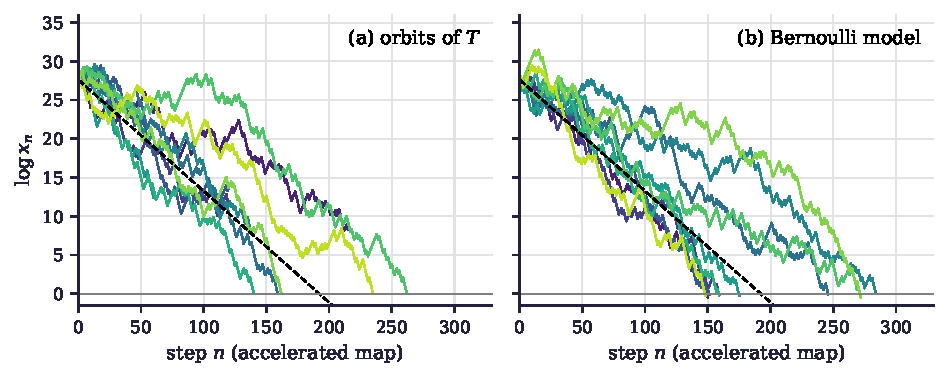
\includegraphics[width=\textwidth]{figures/ch3_paths.pdf}
\caption{Left: $\log x_n$ along ten orbits of the accelerated map started at
odd integers near $10^{12}$. Right: ten paths of the Bernoulli model from the
same height. The dashed line is the mean path $\log x_0+n\ds$.}
\label{fig:ch3:paths}
\end{figure}

\begin{remark}[The constant $14.58$ elsewhere in the book]\label{rem:ch3:c1458}
The number $C=(\log3/\log\frac43)^2$ appears again in \cref{chap:smm}, as the
condition number\index{condition number} at which the Switching MM\index{Switching MM} momentum\index{momentum} coefficient
$\beta=\log(3/2)/\log2$ is the optimal Nesterov\index{Nesterov acceleration} coefficient. This is the same
algebra and not a second piece of evidence: with $\beta=\lt-1$ one has
$(1+\beta)/(1-\beta)=\log3/\log\frac43$ exactly.
\end{remark}

\paragraph{The tail of the stopping time.} The first time $\nu$ at which a
model path falls below its starting height, the model counterpart of the
stopping time $\sigma(n)$ of the map, satisfies
$\Prob(\nu>n)\le\Prob(S_n\ge0)\le\E[e^{\theta S_n}]=M(\theta)^n$ for every
$\theta>0$, by Markov's inequality (this $\theta$ is not the $\theta$ of \cref{thm:density}). The minimum of $M$ is attained at
$\theta=\log(\log2/\log\frac32)/\log3\approx0.4881$, where
$M(\theta)\approx0.9659$. Thus $\Prob(\nu>n)\le0.9659^n$. This is the bound
$e^{-Dk}$ of \cref{thm:density}, obtained there by a Chernoff\index{large deviations} argument for the
binomial count of odd steps; the two computations are the same optimization in
different coordinates, since \cref{prop:ch3:exact} identifies the binomial
count with the number of factors $\tfrac32$ in the model.

\section{The central limit theorem for total stopping times}\label{sec:ch3:clt}

Wald's identity\index{Wald identity} gives the mean of $\tau$; the central limit theorem\index{central limit theorem} for first
passage times gives its fluctuations. For a random walk whose increments have
mean $\mu<0$ and variance $\sigma^2$, the first passage time
$\tau_u=\inf\{n:S_n\le-u\}$ satisfies, as $u\to\infty$,
\begin{equation}\label{eq:ch3:clt}
  \frac{\tau_u-u/|\mu|}{\sqrt{\sigma^2u/|\mu|^3}}\;\Longrightarrow\;N(0,1).
\end{equation}
This is a classical consequence of Anscombe's theorem and the central limit
theorem for the walk; see Gut~\cite{gut1988} for a complete treatment. A limit
in distribution does not by itself give the moments: that $\E[\tau_u]\sim u/|\mu|$
and $\Var(\tau_u)\sim\sigma^2u/|\mu|^3$ is the classical first passage
asymptotics of Heyde\index{Heyde, C. C.}~\cite{heyde1967} and
Siegmund\index{Siegmund, D.}~\cite{siegmund1969} (see
\cite[Theorem~III.9.1]{gut1988}). The
heuristic is quickly told. At time $t=u/|\mu|$ the walk sits at $-u$ plus a
fluctuation of order $\sigma\sqrt t$, and closing that gap at speed $|\mu|$
takes an extra time of order $\sigma\sqrt t/|\mu|$, whose variance is
$\sigma^2t/\mu^2=\sigma^2u/|\mu|^3$.

With $u=\log x_0$, $\mu=\ds$ and $\sigma^2=\frac14(\log3)^2$, the passage time
$\tau_u$ is the time $\tau$ of \cref{prop:lyapunov}, and the model
predicts that it is approximately normal with mean
$\gamma_0\log x_0$ and variance $\sigma^2\log x_0/|\ds|^3\approx101.4\log x_0$.
For this model the normal limit with exactly these constants was proved by
Borovkov\index{Borovkov, K. A.} and Pfeifer\index{Pfeifer, D.}~\cite[Theorem~5]{borovkov2001}.
Both constants are fixed by the drift and the variance of a single step, so the
prediction has no free parameter.
The ratio of the variance to the mean is $C=\sigma^2/(\ds)^2\approx14.58$,
which explains the name index of dispersion in \cref{prop:lyapunov}.
The counterpart of $\tau$ for the map is the total stopping time\index{stopping time}
$\sigma_\infty(n)$ of $T$, the number of steps of $T$ that take $n$ to $1$ (in
\cref{chap:intro} the same symbol counts steps of $T_0$). It is a deterministic
integer, and what can be compared with the law of $\tau$ is its spread over
many starting values $n$.

\begin{table}[t]
\centering
\caption{Total stopping time $\sigma_\infty(n)$ of the accelerated map for
$4000$ starting values $n$ drawn independently and uniformly from each range,
against the leading terms of the Bernoulli model, $\gamma_0\log n$ for the mean (a lower bound for the model mean, by \eqref{eq:ch3:waldbound}) and $101.4\log n$ for the variance, averaged over the sample.}
\label{tab:ch3:clt}
\small
\begin{tabular}{@{}lrrrrr@{}}
\toprule
Range of $n$ & Mean & $\gamma_0\log n$ & Variance & $101.4\log n$ & Ratio\\
\midrule
$[10^3,2\cdot10^3)$ & $49.66$ & $50.73$ & $685.3$ & $739.8$ & $0.926$\\
$[10^4,2\cdot10^4)$ & $65.36$ & $66.69$ & $871.2$ & $972.6$ & $0.896$\\
$[10^5,2\cdot10^5)$ & $81.18$ & $82.76$ & $1101.8$ & $1206.9$ & $0.913$\\
$[10^6,2\cdot10^6)$ & $96.90$ & $98.74$ & $1292.5$ & $1440.0$ & $0.898$\\
$[10^7,2\cdot10^7)$ & $114.33$ & $114.71$ & $1538.3$ & $1672.9$ & $0.920$\\
\bottomrule
\end{tabular}
\end{table}

\Cref{tab:ch3:clt} tests both predictions on samples of $4000$ starting values
drawn independently and uniformly, of either parity, from five ranges
(consecutive integers would not give independent samples, since their orbits
share their tails).
The means fall short of $\gamma_0\log n$ by $0.4$ to $1.8$ steps, whereas by \eqref{eq:ch3:waldbound} the model mean lies above $\gamma_0\log n$, and the overshoot of the barrier puts it $2.07$ steps higher in every range (script \texttt{ch3\_model\_means.py}).
So the real orbits are shorter than model paths from the same height, by $2.5$ to $3.9$ steps in these samples, whose means have standard errors of $0.4$ to $0.6$, and by $3.5$ steps in the exact census at $k=29$ of \cref{sec:ch3:missing}; the overshoot does not explain the shortfall but adds to it.
It is a boundary effect at the end of the orbit: a
real orbit stops on hitting $1$ exactly, with no overshoot, and small integers such as the powers
of two descend to $1$ faster than a random walk from the same height would.
(The $+1$ acts in the opposite direction, lengthening orbits by about one step on average, almost all of it in the final descent; see \cref{sec:ch3:missing}.)
The variances are about $0.9$ times the leading term $101.4\log n$ in every range; the exact variance of the model exceeds its leading term by $2$ to $4$ percent at these sizes, so the variances of the map are $0.87$ to $0.90$ times those of the model, with no clear trend at this sample size; \cref{sec:ch3:missing} locates the deficit exactly.
\Cref{fig:ch3:stopping} shows the regression of total stopping time on $\log n$ and
the pooled standardized residuals
$(\sigma_\infty(n)-\gamma_0\log n)/\sqrt{101.4\log n}$, whose sample variance is $0.909$
and whose skewness is $0.57$; first passage times of a walk with drift\index{drift} are
right skewed at finite $u$, and the skew decays like $u^{-1/2}$.

\begin{figure}[t]
\centering
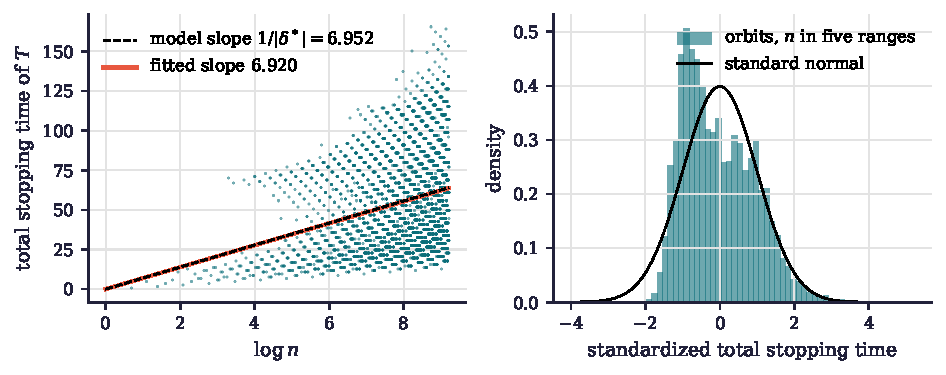
\includegraphics[width=\textwidth]{figures/ch3_stopping.pdf}
\caption{Left: total stopping time of $T$ against $\log n$ for $2\le n\le10^4$,
with the model slope $\gamma_0$ (dashed) and the fitted slope (solid).
Right: standardized total stopping times for $20000$ random $n$ from the five ranges
of \cref{tab:ch3:clt}, against the standard normal density.}
\label{fig:ch3:stopping}
\end{figure}

The conclusion is that the model gets the dispersion of total stopping times right
to about ten percent, erring slightly on the side of too much variability.
There is no excess dispersion to explain. This matters because it is easy to
construct a wrong explanation for a discrepancy that is not there; we return to
this in \cref{rem:ch3:variance}.

\section{Where the missing variance lives}\label{sec:ch3:missing}

The ten percent deficit in \cref{tab:ch3:clt} is small, but it is systematic,
and a complete census
locates its source. For every $n<2^{30}$ we computed the total stopping time\index{stopping time}
$\sigma_\infty(n)$ of $T$ and the number $a(n)$ of odd steps on the way to $1$ (script
\texttt{ch3\_o4\_decomp.py}, which takes about two minutes), and analysed each
dyadic block $[2^k,2^{k+1})$ exactly, not by sampling. The analysis rests on an
identity that holds orbit by orbit.

\begin{proposition}[Pathwise decomposition]\label{prop:ch3:pathwise}
For every $n\ge2$ whose orbit reaches $1$ (as every $n<2^{30}$ of the census does), with $u=\log n$ and $|\ds|=\log(2/\sqrt3)$,
\begin{gather*}
  |\ds|\,\sigma_\infty(n)=u+R(n)+Z(n),\\
  R=\sigma_\infty\log2-a\log3-u,\qquad Z=\tfrac12\log3\,(2a-\sigma_\infty).
\end{gather*}
Here $Z$ is the centred parity sum, a sum of $\sigma_\infty$ terms $\pm\frac12\log3$, and
$R=\sum_{\text{odd steps}}\log(1+1/(3x_i))\ge0$ is the total contribution of the
$+1$ terms. Splitting $Z=Z_{\mathrm h}+Z_{\mathrm t}$ into the sums over the first
$k$ steps and over the rest, for $n$ uniform in $[2^k,2^{k+1})$ the head
$Z_{\mathrm h}$ is exactly a sum of $k$ independent fair signs, so that
$\Var Z_{\mathrm h}=\sigma^2k$ with $\sigma^2=\frac14(\log3)^2$.
\end{proposition}

\begin{proof}
The identity is algebra: $u+R+Z=\sigma_\infty\log2-a\log3+a\log3-\frac12\sigma_\infty\log3=
\sigma_\infty(\log2-\frac12\log3)$. Taking logarithms along the orbit,
$0=\log1=u+a\log\frac32-(\sigma_\infty-a)\log2+\sum_{\text{odd}}\log(1+1/(3x_i))$, which
identifies $R$ with the sum of the $+1$ corrections. For the head, the block
$[2^k,2^{k+1})$ contains each residue class modulo $2^k$ exactly once, and by
\cref{thm:terras} the first $k$ parities are a bijective function of the class;
so they are uniformly distributed over $\{0,1\}^k$, that is, independent fair
bits.
\end{proof}

In the Bernoulli model\index{Bernoulli model} $Z$ would be a martingale\index{martingale} stopped at $\tau$, with
$\E Z^2=\sigma^2\E\tau$ by Wald's second identity\index{Wald identity}, and $R$ would be a bounded
overshoot; the model variance $\sigma^2\log n/|\ds|^3$ is the leading term of
$\Var(Z)/|\ds|^2$. \Cref{tab:ch3:missing} compares each piece with its model
value.

\begin{table}[ht]
\centering\small
\caption{Exact census of the dyadic blocks $[2^k,2^{k+1})$: mean and variance of
$\sigma_\infty$, the leading term $\sigma^2\E\log n/|\ds|^3$ of the model variance, the head ratio $\Var
Z_{\mathrm h}/(\sigma^2k)$, the tail ratio $\Var Z_{\mathrm t}/(\sigma^2\E(\sigma_\infty-k))$,
and the additive deficit $D_{\mathrm v}=\sigma^2\E(\sigma_\infty-k)-\Var Z_{\mathrm t}$.}
\label{tab:ch3:missing}
\setlength{\tabcolsep}{4pt}
\begin{tabular}{@{}rrrrcccr@{}}
\toprule
$k$ & $\E\sigma_\infty$ & $\Var\sigma_\infty$ & model & ratio & head & tail & $D_{\mathrm v}$ \\
\midrule
$10$ & $50.1$ & $709$ & $742$ & $0.956$ & $1.0000$ & $0.939$ & $0.74$ \\
$15$ & $73.6$ & $977$ & $1093$ & $0.894$ & $1.0000$ & $0.909$ & $1.61$ \\
$20$ & $97.7$ & $1308$ & $1445$ & $0.905$ & $1.0000$ & $0.902$ & $2.30$ \\
$25$ & $121.7$ & $1656$ & $1796$ & $0.922$ & $1.0000$ & $0.914$ & $2.51$ \\
$29$ & $141.0$ & $1938$ & $2077$ & $0.933$ & $1.0000$ & $0.924$ & $2.56$ \\
\bottomrule
\end{tabular}
\end{table}

Three conclusions follow. First, the head is exact, as the proposition
requires, and the plus one term $R$ contributes almost nothing to the variance: its
variance is $0.003$ in every block from $k=10$ on, and its covariance with $Z$
is about $0.05$. (Its mean, about $0.15$ in every block and so contributed almost entirely by the final descent, lengthens orbits by about one step.) The whole deficit lives in the tail parity sum, the part of the
orbit beyond the Terras\index{Terras, R.} horizon.

Second, the deficit is \emph{additive}, not multiplicative. The quantity $D_{\mathrm v}$ grows
from $0.74$ at $k=10$ and levels off near $2.6$ (in units of $\log^2$, about
$124$ squared steps of $T$), while the model variance grows linearly in $k$. So
the ratio of observed to model variance first falls, to a minimum near $0.89$
around $k=15$, and then rises again, to $0.933$ at $k=29$. If $D_{\mathrm v}$ stays bounded,
as the census suggests, the ratio tends to $1$ like $1-c/\log n$, and the model is
asymptotically exact to second order. At $n\approx10^{12}$ a saturated deficit
of $2.6$ would give a ratio of about $0.95$.

Third, the deficit sits at the end of the orbit. Splitting each orbit of a random
sample at the first time it falls below $Y=2^{14}$ (script
\texttt{ch3\_o4\_end.py}), the final segment from below $2^{14}$ down to $1$
contributes a deficit of $1.94$ to $1.98$ for $k=20$, $24$ and $28$, independent
of $k$, and is uncorrelated with what came before; the middle segment, from the
Terras horizon down to $2^{14}$, contributes $0.40$, $0.62$ and $0.64$, with its variance ratio
rising towards $1$ as $k$ grows ($0.914$, $0.930$, $0.952$). The final segment is
a finite deterministic system: every orbit enters $[1,2^{14})$ and then follows
one of finitely many fixed paths to $1$. Those paths are shorter and less
variable than a random walk descending from the same heights, because the
small integers are funnelled into a few common tails, through $20$, $10$, $5$ and the
powers of two. The model treats the last sixty or so steps as fresh coin flips,
and they are not.

So the census indicates that the deficit is a bounded boundary
effect at the bottom of the orbit, plus a smaller contribution from the passage
to the bottom, and that the Bernoulli model is asymptotically right about the
variance; a proof that the deficit stays bounded is the first part of open
problem O4 of \cref{chap:open}. The third cumulant is less well explained: the observed skewness of
$\sigma_\infty$ is $0.62$ at $k=20$ and $0.67$ at $k=29$, while the inverse Gaussian law
of a drifted Brownian first passage, with the model's drift\index{drift} and variance,
predicts $3\sigma/\sqrt{|\ds|\,\E\log n}$, which is $1.15$ and $0.96$. The real
total stopping times are less skewed than the model's passage times, and we leave the explanation
open.

\section{Excursions: the Ville and Lundberg bound}\label{sec:ch3:ville}

How high can an orbit climb before it descends? The orbit of $27$ under $T_0$ climbs to
$9232$, a factor of about $342$ (under $T$ its peak is $4616$), and such excursions are the most visible
feature of the problem. In the model the answer is controlled exactly by the
martingale\index{martingale} property, through a maximal inequality that goes back to
Ville\index{Ville inequality}\index{Ville, J.}~\cite{ville1939}.

\begin{proposition}[Ville bound]\label{prop:ch3:ville}
In the Bernoulli model\index{Bernoulli model} for $T$, for every $x_0>0$ and $K\geq1$,
\[
  \Prob\Bigl(\sup_{n\geq0}x_n\geq Kx_0\Bigr)\;\le\;\frac1K .
\]
Equivalently, in terms of the log walk, $\Prob(\sup_nS_n\geq u)\le e^{-u}$ for
every $u\geq0$. The same bound holds in the stride model for $S$, and in the
renewal\index{renewal theory} model for $T_0$ when $B_0=0$; when $B_0=1$ the bound becomes $3/K$.
\end{proposition}

\begin{proof}
Let $c=Kx_0$ and $\eta=\inf\{n:x_n\geq c\}$. The stopped process
$x_{n\wedge\eta}$ is a nonnegative martingale, so for each $n$
\[
  x_0=\E[x_{n\wedge\eta}]\geq\E[x_\eta;\eta\le n]\geq c\,\Prob(\eta\le n).
\]
Letting $n\to\infty$ gives $\Prob(\eta<\infty)\le x_0/c=1/K$. For the stride
model apply the same argument to the martingale $X_j$; the supremum over
strides is the supremum over odd values, which is the relevant one. For the
renewal model apply it to $M_n=3^{B_n}x_n\geq x_n$, whose initial value is
$3^{B_0}x_0$.
\end{proof}

The proposition is the Lundberg inequality of risk theory in the special case
$\theta^*=1$. For a general walk with negative drift\index{drift} the bound reads
$\Prob(\sup_nS_n\geq u)\le e^{-\theta^*u}$, and the Cram\'er and Lundberg
approximation sharpens it to $\Prob(\sup_nS_n\geq u)\sim C_{\mathrm L}e^{-\theta^*u}$ for a
constant $C_{\mathrm L}<1$ that depends on the overshoot over the level~\cite{asmussen2010}.
For the Collatz model this says that $K\cdot\Prob(\sup x_n\geq Kx_0)$ should
settle to a constant a little below one.

\Cref{fig:ch3:ville} tests the bound. For each $n$ with $2\le n\le10^6$ we
computed the maximum of the orbit of $n$ under $T$ and recorded the fraction of
$n$ whose maximum is at least $Kn$, for $K=2,4,\ldots,4096$. The product $K$
times this fraction lies between $0.76$ and $0.85$ for $K\le1024$, comfortably
below the bound. A simulation of $10^6$ paths of the Bernoulli model gives
values between $0.82$ and $0.85$ over the same range, an estimate of the
Cram\'er and Lundberg constant. The orbits sit a little below the model, in
line with the slightly smaller dispersion found in \cref{sec:ch3:clt}. The drop
at $K=2048$ and $K=4096$ is an edge effect: at these factors only a few hundred
of the million starting values qualify, and the integers below $10^6$ are too
small for the orbit to have room to make such excursions in the proportion the
model predicts.

\begin{figure}[t]
\centering
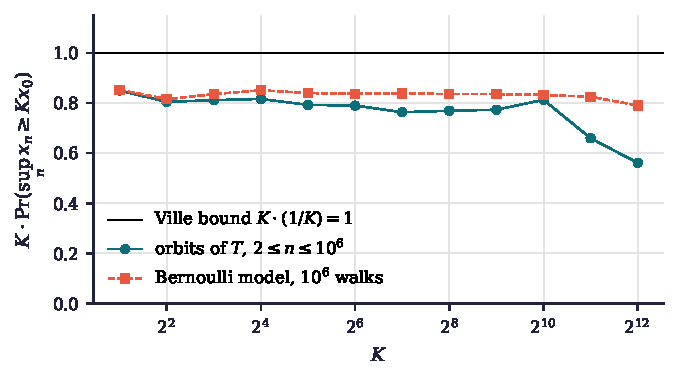
\includegraphics[width=\textwidth]{figures/ch3_ville.pdf}
\caption{The quantity $K\cdot\Prob(\sup_nx_n\geq Kx_0)$ for orbits of $T$
with $2\le n\le10^6$ (circles) and for $10^6$ paths of the Bernoulli model
(squares). For the model, Ville's inequality (\cref{prop:ch3:ville}) says that it never exceeds $1$.}
\label{fig:ch3:ville}
\end{figure}

\paragraph{The exponent $2$.} The Ville bound explains a prediction of
Lagarias\index{Lagarias, J. C.} and Weiss\index{Weiss, A.}~\cite{lagarias1992} about the maximal excursion
$t(n)=\max_kT^{(k)}(n)$. Treat the orbits of different $n$ as independent
model paths. Taking $K=n^{1+\varepsilon}$ gives
$\Prob(t(n)\geq n^{2+\varepsilon})\le n^{-1-\varepsilon}$, which is summable,
so by the Borel and Cantelli lemma only finitely many $n$ would have
$t(n)\geq n^{2+\varepsilon}$. In the other direction the Cram\'er and Lundberg
asymptotics give $\Prob(t(n)\geq n^{2-\varepsilon})\approx C_{\mathrm L}n^{-1+\varepsilon}$,
which is not summable, and independence would give infinitely many such $n$.
The heuristic conclusion is $\limsup_n\log t(n)/\log n=2$. Over
$1000<n\le10^6$ the largest value of $\log t(n)/\log n$ for the accelerated map\index{accelerated map}
is $1.9095$, attained at $n=159487$. The heuristic is of course only as good
as the independence assumption, which is false for neighbouring integers whose
orbits merge, and there is no proof that $t(n)\le n^{C}$ for any constant $C$.

\section{Parity autocorrelations}\label{sec:ch3:autocorr}

Under the accelerated map\index{accelerated map} the model parities are independent. Under the
standard map\index{standard map} they are not, and their dependence can be computed exactly.

\begin{proposition}[Parity autocorrelation function]\label{thm:autocorr}
In the renewal\index{renewal theory} model for $T_0$, started from its stationary law, the model
parity chain $(B_n)$ is stationary with
\[
  \Prob(B_n=1)=\frac{1}{1+\E[K]}=\frac13,\qquad\Var(B_n)=\frac29,
\]
and its autocorrelation\index{autocorrelation} function is
\begin{equation}\label{eq:ch3:rhoh}
  \rho(h)=\mathrm{Corr}(B_n,B_{n+h})=\Bigl(-\frac12\Bigr)^{h},\qquad h\geq0 .
\end{equation}
\end{proposition}

\begin{proof}
We give the renewal proof, which explains where the formula comes from; a
second proof is in \cref{rem:ch3:markov}. By
\cref{prop:ch3:standard}(v), the gaps between successive ones of $(B_n)$ are
independent copies of $G=1+K$, with
\[
  \Prob(G=m)=\Prob(K=m-1)=2^{-(m-1)},\qquad m\geq2 .
\]
Hence $\E[G]=1+\E[K]=3$, and by the renewal theorem the stationary probability
of a one is $1/\E[G]=\frac13$, so $\Var(B_n)=\frac13\cdot\frac23=\frac29$. The
generating function of the gap law is
\[
  F(z)=\sum_{m\geq2}2^{-(m-1)}z^m=\frac{z^2}{2-z},\qquad|z|<2 .
\]
Let $u(h)=\Prob(B_{n+h}=1\mid B_n=1)$ be the renewal sequence, with $u(0)=1$.
Decomposing according to the time of the first renewal after time $n$ gives the
renewal equation $u(h)=\sum_{m=1}^{h}\Prob(G=m)u(h-m)$ for $h\geq1$, which in
generating functions reads $U(z)=1+F(z)U(z)$, where
$U(z)=\sum_{h\geq0}u(h)z^h$. Therefore
\[
  U(z)=\frac{1}{1-F(z)}=\frac{2-z}{2-z-z^2}=\frac{2-z}{(1-z)(2+z)} .
\]
Partial fractions give
\[
  U(z)=\frac{1/3}{1-z}+\frac{4/3}{2+z}
      =\frac{1/3}{1-z}+\frac{2/3}{1+z/2},
\]
and expanding both terms as geometric series,
\begin{equation}\label{eq:ch3:renewal}
  u(h)=\frac13+\frac23\Bigl(-\frac12\Bigr)^{h},\qquad h\geq0 .
\end{equation}
The first values are $u(0)=1$, $u(1)=0$, $u(2)=\frac12$, $u(3)=\frac14$,
$u(4)=\frac38$. Finally, with $p=\frac13$,
\begin{align*}
  \rho(h)&=\frac{\Prob(B_n=1,B_{n+h}=1)-p^2}{p(1-p)}=\frac{p\,u(h)-p^2}{p(1-p)}\\
  &=\frac{u(h)-p}{1-p}=\frac32\Bigl(u(h)-\frac13\Bigr)=\Bigl(-\frac12\Bigr)^{h}. \qedhere
\end{align*}
\end{proof}

The first three values of the renewal sequence carry the arithmetic of a single stride.
$u(1)=0$ is \cref{prop:nocons}: there are never two consecutive odd steps.
$u(2)=\tfrac12$ and $u(3)=\tfrac14$ are the probabilities that the halving exponent equals $1$ and $2$, that is $\Prob(x\equiv3\pmod4)$ and $\Prob(x\equiv1\pmod8)$ for odd $x$ (\cref{prop:geom}).
From $h=4$ on the values involve the joint law of successive halving exponents, beginning with $u(4)=\Prob(K=3)+\Prob(K=1)^2=\tfrac38$; that law is exact for random residues over the range of \cref{prop:ch3:exact}, and beyond it the independence of successive exponents is an assumption of the model.

\begin{remark}[A second proof]\label{rem:ch3:markov}
Since $(B_n)$ is a Markov chain with transition matrix $P$, the conditional
law of $B_{n+h}$ given $B_n$ is given by $P^h$. Writing $P=\Pi+(-\tfrac12)E$ with
$\Pi$ the rank one projection onto the stationary vector and $E$ the
complementary spectral projection, $P^h=\Pi+(-\tfrac12)^hE$, and the
autocorrelation of any function of a reversible two state chain decays like
the $h$th power of the second eigenvalue. The renewal proof has the advantage
of exhibiting the generating function $U(z)$, which is what one needs for
the variance computation below.
\end{remark}

\begin{corollary}[Long run variance of the log path]\label{cor:longrun}
In the renewal model for $T_0$, the autocorrelation factor is
\[
  \mathcal{A}:=1+2\sum_{h\geq1}\rho(h)=1+2\cdot\frac{-1/2}{1+1/2}=\frac13 ,
\]
and the variance of the log path satisfies
\[
  \frac{\Var(\log x_n)}{n}\;\longrightarrow\;\mathcal{A}\cdot\frac29(\log6)^2
  =\frac{2}{27}(\log6)^2\approx0.2378 .
\]
\end{corollary}

\begin{proof}
The log increment at step $n$ is $B_n\log3-(1-B_n)\log2=B_n\log6-\log2$, a
linear function of $B_n$ with slope $\log6$. For a stationary sequence with
summable autocovariances we have
$\Var(\sum_{i<n}B_i)/n\to\Var(B)\,\mathcal{A}$.
The same limit holds from any initial state: the parities form a two state Markov chain whose second eigenvalue is $-\tfrac12$, so the law of $B_i$ approaches the stationary law geometrically fast, which changes $\Var(\sum_{i<n}B_i)$ by $O(1)$.
Here $\Var(B)=\frac29$ and $\sum_{h\geq1}(-\tfrac12)^h=-\tfrac13$, so
$\mathcal{A}=\frac13$ and the limit is $\frac13\cdot\frac29(\log6)^2$. As a
check, the variance asymptotic of renewal theory~\cite[Theorem~III.9.1]{gut1988} says that the
number $a_n$ of renewals before time $n$ has
$\Var(a_n)/n\to\Var(G)/\E[G]^3=2/27$, since $\Var(G)=\Var(K)=2$ and
$\E[G]=3$; and $\log x_n=\log x_0+a_n\log6-n\log2$. The two routes agree.
\end{proof}

\Cref{cor:longrun} has a consequence that runs against a natural intuition.

\begin{remark}[A tempting but false argument]\label{rem:ch3:variance}
One might argue as follows: ``the parities of $T_0$ are correlated, correlated
increments make a random walk more variable than an independent one, and so
the parity correlations should inflate the dispersion of total stopping times\index{stopping time} well
beyond what an independent model predicts.'' Each clause sounds reasonable, and
the conclusion is wrong in sign. The correlations are negative at odd lags and
alternate, $\rho(h)=(-\frac12)^h$, and their sum is $-\frac13$. The long run
variance factor is $\mathcal{A}=\frac13<1$, so the correlations \emph{reduce}
the variance of the log path by a factor of three relative to an independent
sequence with the same marginal law. Negative lag one correlation is exactly
what one expects from a forced halving after every tripling: an up step is
always cancelled in part by the next step. Two further facts close the
question. First, measured on the clock of $T$, where the model parities are
independent, the reduction disappears and what remains is the variance
$\sigma^2$ of \cref{prop:lyapunov}; the factor $\frac13$ and the deletion of
forced steps are two descriptions of the same thing. So $\mathcal{A}$ concerns
only the log path of $T_0$ counted in its own steps, and parity correlations
play no part in the dispersion law of \cref{sec:ch3:clt}, which is stated on
the clock of $T$. Second, as
\cref{tab:ch3:clt} shows, there is no excess dispersion of total stopping times to
explain: the observed variance is about $0.9$ of the model value. Any
mechanism that predicts an inflation of the variance by a large factor, from
parity correlations or from anything else, is contradicted by the data.
\end{remark}

\subsection{The empirical check}

\Cref{fig:ch3:acf} compares \eqref{eq:ch3:rhoh} with two empirical
autocorrelation\index{autocorrelation} functions for the parity sequence $b_j$ of $T_0$, both
estimated with the mean and variance pooled over all recorded steps: if $\hat p$
is the fraction of odd steps, the estimate at lag $h$ is
$(\overline{b_jb_{j+h}}-\hat p^{\,2})/(\hat p(1-\hat p))$, where the bar is the
average over all recorded pairs of steps $h$ apart. The first is a scan
over small starting values: orbits started at $27$ and then restarted at a
random odd number below $10^4$ each time they reach $1$, for a total of
$4\times10^5$ steps. These orbits are not truncated but followed all the way to
$1$. The fraction of odd steps is $0.3351$ and the first six lags are
\[
  -0.5040,\quad+0.2482,\quad-0.1530,\quad+0.0822,\quad-0.0032,\quad-0.0139,
\]
against the predicted values $(-\tfrac12)^h$, that is $-0.5$, $+0.25$, $-0.125$,
$+0.0625$, $-0.0313$ and $+0.0156$.
The first two lags agree (at lag one this is forced: no two odd steps are consecutive, so the estimate is $-\hat p/(1-\hat p)$ whatever the orbits).
From lag three on the agreement is visibly worse, and lag six even has the wrong sign.
Lag three still reflects a single stride: the halving exponent $2$, which has probability $u(3)=\tfrac14$ in the model, occurs in only $23.3$ percent of the strides of the scan. We regard
this as a genuine feature of short orbits and not as sampling noise. Small
starting values have few bits, so most of each orbit lies outside the range of
\cref{prop:ch3:exact}, and the scan includes the final descent of every orbit
through the powers of two and the cycle $4\to2\to1$, whose parity pattern is
far from stationary.

The second check uses large starting values and truncated orbits. For $4000$
random integers $n$ between $2^{200}$ and $2^{208}$, of either parity and with
$n\bmod2^{200}$ uniformly distributed, we recorded the parities of steps $50$ to
$299$ of $T_0$, far above the trivial cycle. By \cref{prop:ch3:exact} all but
about one percent of these steps lie inside the range in
which the parities of $T$ are exactly independent and fair, so apart from that
one percent and from sampling error the model is a theorem here. The fraction of odd steps is $0.3330$, and
the autocorrelations are $-0.4993$, $+0.2497$, $-0.1252$, $+0.0629$,
$-0.0320$, $+0.0155$ for $h=1,\ldots,6$, in agreement with $(-\tfrac12)^h$ to
the precision of the sample. The renewal\index{renewal theory}
formula is exact for an ensemble of starting values over the initial segment
of their orbits; along the late part of short orbits it is a prediction, and
the prediction is visibly imperfect from lag three on.

\begin{figure}[t]
\centering
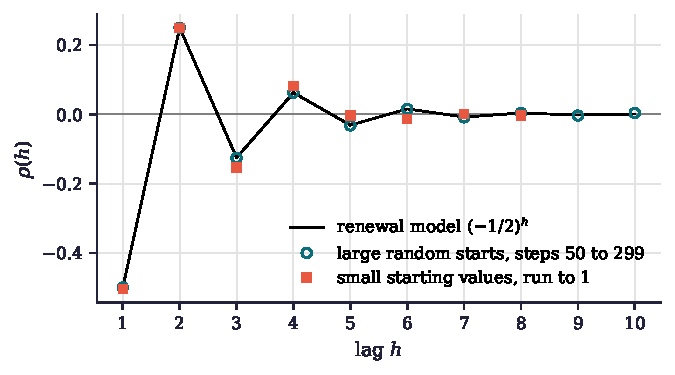
\includegraphics[width=\textwidth]{figures/ch3_acf.pdf}
\caption{Autocorrelation of the parity sequence of the standard map, estimated
with the pooled mean and variance. Solid
line: the renewal model $(-\tfrac12)^h$. Circles: $4000$ large random starting
values of either parity, steps $50$ to $299$. Squares: small odd starting values, orbits run to
$1$.}
\label{fig:ch3:acf}
\end{figure}

\section[Absorption and the failure of uniform integrability]{Absorption and the failure of\\ uniform integrability}\label{sec:ch3:absorb}

We now come to the two results that locate the obstruction precisely. The
first says that the model settles its own version of the conjecture. The
second says why the martingale\index{martingale} of \cref{thm:martingale} cannot be used to
settle it, even in the model.

\begin{proposition}[The model absorbs almost surely]\label{prop:absorb}
Let $\Delta_1,\Delta_2,\ldots$ be independent and identically distributed and
integrable with mean $\mu<0$, and put $\log x_n=\log x_0+\sum_{i\le n}\Delta_i$
with $x_0>1$. Let $\tau=\inf\{n:x_n\le1\}$. Then $\E[\tau]<\infty$; in
particular
\[
  \Prob\bigl(x_n>1\text{ for all }n\bigr)=0 .
\]
If moreover $\Delta_i\geq-L$ almost surely, then
$\E[\tau]<(\log x_0+L)/|\mu|$.
\end{proposition}

\begin{proof}
Suppose first that $\Delta_i\geq-L$. The process $N_n=\log x_n-n\mu$ is a
martingale, and optional stopping at the bounded time $n\wedge\tau$ gives
\[
  \E[\log x_{n\wedge\tau}]=\log x_0+\mu\,\E[n\wedge\tau] .
\]
Before time $\tau$ the value $\log x$ is positive, and at time $\tau$ it is at
least $\log x_{\tau-1}-L>-L$. Hence $\log x_{n\wedge\tau}>-L$, and
$|\mu|\,\E[n\wedge\tau]<\log x_0+L$. Monotone convergence as $n\to\infty$ gives
$|\mu|\,\E[\tau]\le\log x_0+L$.
So $\tau$ is integrable, Wald's identity\index{Wald identity} $\E[\log x_\tau]=\log x_0+\mu\,\E[\tau]$ holds, and since $\log x_\tau>-L$ almost surely the bound is strict.

In general, put $\Delta_i'=\max(\Delta_i,-L)$. As $L\to\infty$,
$\E[\Delta_i']$ decreases to $\mu$ by monotone convergence, so we may fix $L$
with $\mu'=\E[\Delta_i']<0$. The walk built from the $\Delta_i'$ lies above the
original walk, so its passage time $\tau'$ below $0$ satisfies
$\tau\le\tau'$, and by the first part $\E[\tau']<(\log x_0+L)/|\mu'|$. In
either case $\tau$ is integrable and therefore finite almost surely.
\end{proof}

For the Bernoulli model\index{Bernoulli model} $L=\log2$ and the bound is the upper half of
\eqref{eq:ch3:waldbound}. For the stride model the downward steps
$\log3-K\log2$ are unbounded, and the truncation in the second half of the
proof is needed.

The proposition is the strong law of large numbers in martingale dress, and the
dress is the point. Its only inputs are a negative mean and independence of the
increments from the past, which is what makes $N_n$ a martingale. For the
Collatz map the increments are deterministic functions of the current iterate,
there is no filtration with respect to which $\log x_n-n\ds$ is a martingale,
and \cref{prop:absorb} has no analogue. The Ces\`aro liminf conjecture of
\cref{chap:divergence} asks for a deterministic substitute for the part of this argument that excludes escape to infinity; it says nothing about cycles.

\begin{proposition}[Failure of uniform integrability]\label{prop:uimartingale}
In the Bernoulli model for $T$ with $x_0>1$, let $\tau=\inf\{n:x_n\le1\}$. Then
$\tau<\infty$ almost surely, the stopped process $(x_{n\wedge\tau})_{n\geq0}$ is
a nonnegative martingale converging almost surely to $x_\tau\le1$, and it is
not uniformly integrable\index{uniform integrability}. More precisely, for every $n$,
\[
  \E\bigl[x_n;\tau>n\bigr]\;\geq\;x_0-1,\qquad\text{while}\qquad
  \Prob(\tau>n)\to0 .
\]
\end{proposition}

\begin{proof}
Almost sure finiteness of $\tau$ is \cref{prop:absorb}. The stopped process of a
martingale is a martingale, so $\E[x_{n\wedge\tau}]=x_0$ for every $n$, and
\[
  x_0=\E[x_\tau;\tau\le n]+\E[x_n;\tau>n]\le\Prob(\tau\le n)+\E[x_n;\tau>n],
\]
which gives the first inequality. If the stopped process were uniformly
integrable, then $x_{n\wedge\tau}\to x_\tau$ in $L^1$, and
$x_0=\lim\E[x_{n\wedge\tau}]=\E[x_\tau]\le1$, a contradiction. Equivalently,
the expectations $\E[x_n;\tau>n]$ stay above $x_0-1>0$ on events whose
probabilities tend to zero, which is exactly the failure of uniform
integrability.
\end{proof}

The two propositions are consistent and together they locate the
obstruction. The martingale $(x_n)$ has constant mean $x_0$ while almost every
path is absorbed. The mass that keeps the mean up escapes along the rare paths
that have not yet been absorbed, and these paths carry, at every time $n$, an
expected value of at least $x_0-1$. Taking logarithms converts the martingale
into a supermartingale\index{supermartingale} with drift\index{drift}, which is why \cref{prop:absorb} works for
$\log x$ and cannot be run for $x$. The power functions $x^\theta$ with
$0<\theta<1$ sit in between: by \cref{thm:martingale}(iii) they are
supermartingales with geometric drift $M(\theta)<1$, and they are the model
counterpart of the power majorizer\index{majorization}s of \cref{chap:lyapunov}.

\begin{remark}[What a certificate would have to be]\label{rem:ch3:cert}
Suppose we tried to turn the model into a proof. In a probabilistic setting
one would look for a uniformly integrable martingale $Y_n$ that converges to the
indicator of absorption; then $Y_0=\Prob(\tau<\infty)$, and showing $Y_0=1$ is
the statement to be proved. Such a martingale always exists, namely
$Y_n=\Prob(\tau<\infty\mid\Filt_n)$, but writing it down requires knowing the
absorption probability, which is the thing to be proved; in the model it is
identically $1$ by \cref{prop:absorb}, so the certificate\index{certificate} is trivial and
uninformative. In the model the only martingales of the form $x_n^\theta$ are
those with $\theta=0$ and $\theta=1$, the roots of $M(\theta)=1$ in
\cref{thm:martingale}, and neither carries information about termination.

For the deterministic map the analogue of the conditional probability is the
function $h(x)=1$ if the orbit of $x$ reaches $1$ and $h(x)=0$ otherwise. It is
invariant, $h(T(x))=h(x)$, and the conjecture is the assertion $h\equiv1$. A
useful certificate would be a computable function $g\ge0$ that decreases along
orbits by a definite amount away from $1$, and \cref{chap:lyapunov} shows that
no such function that increases with $x$ exists, whatever fixed number of
strides is allowed for the decrease (\cref{thm:nolyapunov,cor:ch4:multistride}). What the model
offers instead is decrease in expectation, and expectation requires a measure.
The only measures for which the Collatz parities are provably independent are
the uniform measures on residue classes of \cref{prop:ch3:exact}, and they
control a single orbit for only as many steps as the residue class has bits. A
certificate along these lines would therefore have to show that the
information an orbit generates as it proceeds is, in a quantitative sense,
as good as fresh randomness. This is the content of the equidistribution\index{equidistribution}
questions of \cref{chap:divergence}, and it is where every known approach
stops.
\end{remark}

\section*{Notes}

\Cref{sec:ch3:heuristic} tells the history of the model; the survey of Kontorovich\index{Kontorovich, A. V.} and Lagarias~\cite{kontorovich2009} is the best general reference for stochastic models of the $3x+1$ and $5x+1$ problems. The presentation of
the martingale\index{martingale}
duality of \cref{thm:martingale}, the martingale $3^{B_n}x_n$ for the standard
map and the renewal computation of $\rho(h)=(-\tfrac12)^h$ and $\mathcal{A}=\frac13$
is ours, but all of these are elementary, and the closed form is the
autocorrelation of a two state Markov chain; the renewal\index{renewal theory} structure of the model parity
sequence is implicit in all treatments that use the Geometric law of the
halving exponent. The dispersion law of \cref{sec:ch3:clt} is the classical
first passage asymptotics of Heyde\index{Heyde, C. C.}~\cite{heyde1967} and
Siegmund\index{Siegmund, D.}~\cite{siegmund1969}; for this model
Borovkov\index{Borovkov, K. A.} and Pfeifer\index{Pfeifer, D.}~\cite[Theorem~5]{borovkov2001}
proved the normal limit with these constants.

For martingales, optional stopping and the convergence theorems we have used,
Williams\index{Williams, D.}~\cite{williams1991} is a concise and elegant source. Wald's identity\index{Wald identity}
is from Wald\index{Wald, A.}~\cite{wald1944}; the maximal inequality for nonnegative
supermartingales\index{supermartingale} appears in Ville\index{Ville inequality}\index{Ville, J.}'s thesis~\cite{ville1939}, which also
introduced the word martingale into probability. Renewal theory, the renewal
central limit theorem\index{central limit theorem} and the ladder variables behind the Cram\'er and Lundberg
approximation are in Feller\index{Feller, W.}~\cite{feller1971}; Gut\index{Gut, A.}~\cite{gut1988} treats
first passage times and Anscombe's theorem; Asmussen\index{Asmussen, S.} and
Albrecher\index{Albrecher, H.}~\cite{asmussen2010} is the standard reference for Lundberg
inequalities in risk theory, where the Wald root is called the adjustment
coefficient.

\begin{sloppypar}
All numerical results in this chapter were computed by the authors; the scripts
are \texttt{ch3\_stats.py}, \texttt{ch3\_stopping.py},
\texttt{ch3\_figures.py}, \texttt{ch3\_o4\_decomp.py}, \texttt{ch3\_o4\_census.py} and \texttt{ch3\_o4\_end.py} in the code appendix; the exact moments of the model passage time come from \texttt{ch3\_model\_means.py}, which uses \texttt{ch3\_o4\_model.py}.
\end{sloppypar}

\section*{Exercises}

\begin{exercise}\label{ex:ch3:fivex}
Repeat the computations of \cref{thm:martingale} for the $5x+1$ map, with
accelerated form $x\mapsto(5x+1)/2$ for odd $x$. Show that the log drift\index{drift} under
the fair coin model is $\frac12\log\frac54>0$, that the factors no longer have
mean one, and find the nonzero root of the moment generating function. What
does the sign of the root say about excursions?
\end{exercise}

\begin{exercise}\label{ex:ch3:wald}
In the stride model, let $\tau$ be the first stride at which $X_j\le1$. Use
Wald's identity\index{Wald identity} to show that $\E[\tau]=\log X_0/\log\frac43+O(1)$, and
reconcile this with the slope $\gamma_0$ of \cref{prop:lyapunov} by counting
steps of $T$ per stride.
\end{exercise}

\begin{exercise}\label{ex:ch3:renewal}
Let the halving exponent have a general law on $\{1,2,\ldots\}$ with
generating function $\phi(z)=\E[z^K]$. Show that the renewal\index{renewal theory} sequence of the
parity chain of $T_0$ has generating function $U(z)=1/(1-z\phi(z))$, and
verify \eqref{eq:ch3:renewal} for $\phi(z)=z/(2-z)$. For which laws of $K$ is
$\rho(2)>0$?
\end{exercise}

\begin{exercise}\label{ex:ch3:ville}
In the Bernoulli model\index{Bernoulli model}, let $\eta$ be the first time $x_n\geq Kx_0$ and
$\zeta$ the first time $x_n\le\varepsilon$, where $0<\varepsilon<x_0$. Apply
optional stopping to the bounded martingale\index{martingale} $x_{n\wedge\eta\wedge\zeta}$, using
the fact that a level is overshot by at most a factor $\frac32$, to show that
\[
  \frac{2}{3K}\;\le\;\Prob\Bigl(\sup_nx_n\geq Kx_0\Bigr)\;\le\;\frac1K .
\]
Thus the Ville\index{Ville inequality} bound is sharp up to a constant factor.
\end{exercise}

\begin{exercise}\label{ex:ch3:standardui}
In the renewal model for $T_0$, let $\tau$ be the first time $x_n\le1$, and suppose that $x_0>1$ and $3^{B_0}x_0>2$, that is, $x_0>2$ or $B_0=1$. Show
that the stopped martingale $M_{n\wedge\tau}$, with $M_n=3^{B_n}x_n$, is not
uniformly integrable\index{uniform integrability}, and that $\E[M_n;\tau>n]\geq3^{B_0}x_0-2$ for every $n$
while $\Prob(\tau>n)\to0$. (Hint: the step into $\tau$ is a halving, so $B_\tau$ is a fair coin independent of the past.) What happens when $B_0=0$ and $1<x_0\le2$?
\end{exercise}

\begin{exercise}\label{ex:ch3:simulate}
Write a program that estimates the Cram\'er and Lundberg constant
$C_{\mathrm L}=\lim_{K\to\infty}K\,\Prob(\sup_nx_n\geq Kx_0)$ for the Bernoulli model, and
compare your estimate with the values near $0.84$ reported in
\cref{sec:ch3:ville}.
\end{exercise}
